\documentclass[12pt]{article}
\usepackage[utf8]{inputenc}

\title{COMP 138 RL: Homework 2}
\author{Erli Cai}

\usepackage{subcaption}
\usepackage{graphicx}
\graphicspath{ {./images/} }
\usepackage[fleqn]{amsmath}
\begin{document}

\maketitle
\setlength\parindent{0pt}


\section{Motivation}
In textbook, we have introduced several methods of estimating value functions and discovering optimal policies, including Dynamic programming and Monte Carlo method. Comparing with dynamic programming method, we need only actual experience but not complete knowledge of environment using Monte Carlo method. This makes Monte Carlo method particularly useful in some cases. In this programming task, we will investigate performance of On-Policy First-Visit Monte Carlo method on finding optimal path for a car in race track.


\section{Background}
\subsection{Monte Carlo Method}
Monte Carlo methods are ways of solving the reinforcement learning problem based on averaging sample returns. When applying Monte Carlo method we do not need to assume complete knowledge of the environment. We just need sample sequences of states, actions, and rewards from actual or simulated interaction with an environment. It is like a bandit problem with the main difference being that now there are multiple states, each acting like a different bandit problem and the different bandit problems are interrelated.


\subsection{Generalized Policy Iteration}
Policy iteration consists of two simultaneous, interacting processes, one making the value function consistent with the current policy (policy evaluation), and the other making the policy greedy with respect to the current value function (policy improvement). We use the term generalized policy iteration (GPI) to refer to the general idea of letting policy evaluation and policy improvement processes interact, independent of the granularity and other details of the two processes. It is easy to see that if both the evaluation process and the improvement process stabilize, that is, no longer produce changes, then the value function and policy must be optimal.

\subsection{On policy method v.s. Off policy method}
To ensure we find the optimal policy, we must ensure that all actions are selected infinitely often. There are two approaches to ensuring this, resulting in on-policy methods and off-policy methods. On-policy methods attempt to evaluate or improve the policy that is used to make decisions, whereas off-policy methods evaluate or improve a policy different from that used to generate the data. Generally, on-policy reinforcement learning is useful when you want to optimize the value of an agent that is exploring. And when the agent does not explore much, off-policy RL may be more appropriate.

\section{Problem Settings and implementation}
In this problem, we are trying to investigate the performance of On-Policy First-Visit Monte Carlo method on finding optimal path for a car in race track. More specifically, we are interested in a race track with a right angle turn(Figure 1 below shows what the track looks like) . The car is assumed to start at random position on a starting line with horizontal velocity and vertical velocity both equal 0 initially. At each time step, velocity in each direction can change by 1,0 or -1. And velocity in each direction should be in between 0 and -5. Apart from that, with probability 0.1 at each time step the velocity increments are both zero, independently of the intended increments. \\

Among different Monte Carlo methods, we choose to implement On-Policy First-Visit Monte Carlo method, which is a $\epsilon $-soft policy, meaning it has $\epsilon$ probability of exploring non-optimal actions. we set reward to be -1 on each time step and we will calculate the average reward of 50 simulations in 1000 steps and use it as a measure of performance.


\pagebreak

\section{Result}
From Figure 2, we can see that the average rewards starts at a very negative value(-700) in the beginning and first fast and them slowly climbs to approximately -100.  This means racecar still needs about 100 time steps to reach finishing line. However, this does not mean our algorithm is not good enough since actual optimal policy takes less than 10 step to reach finishing line(as we shall see below). This only reflex that there are $10\%$ chance the car don't change speed and that the algorithm has a good chance of performing exploration.
\begin{figure}
  \centering
     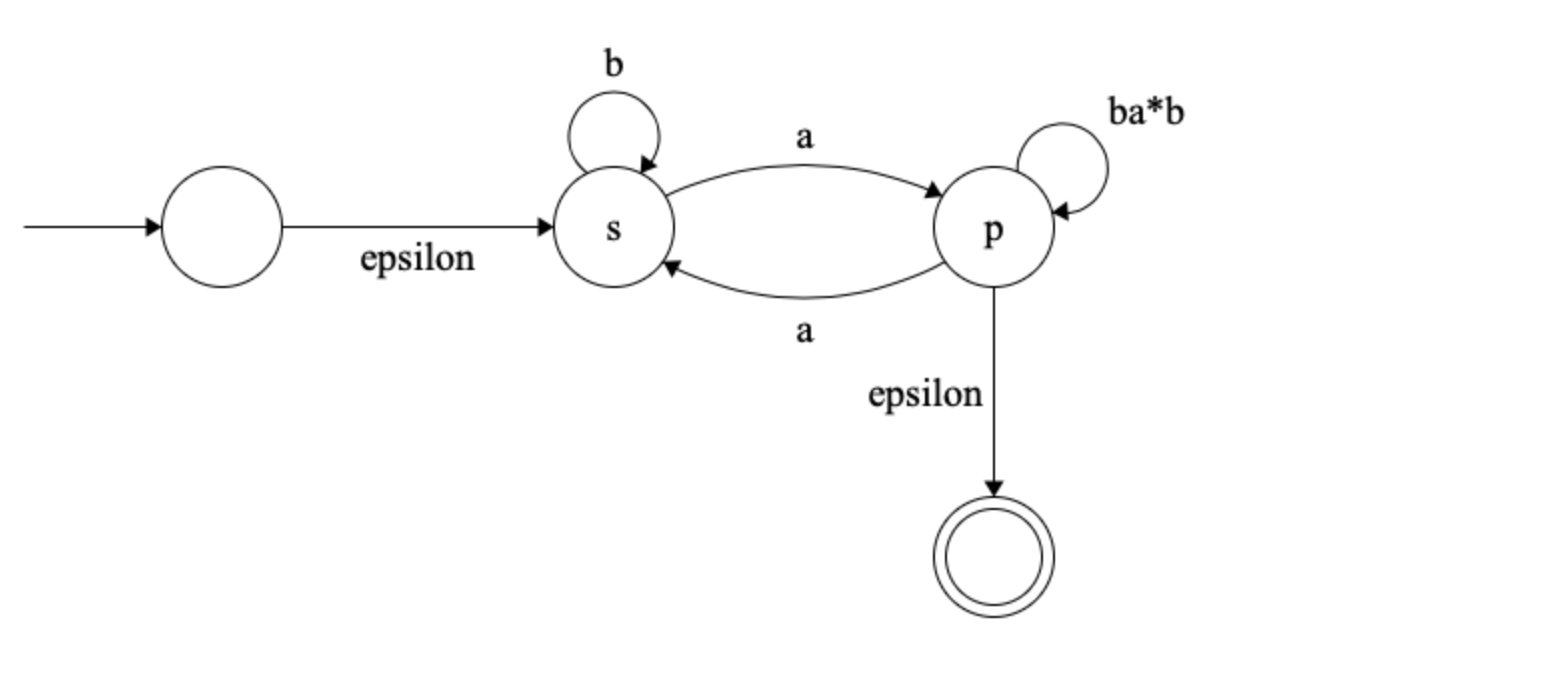
\includegraphics[scale = 0.16]{4.png}
  \caption{Race Track drawn in grid, yellow areas are starting line and finish line}
\end{figure}

\begin{figure}
  \centering
     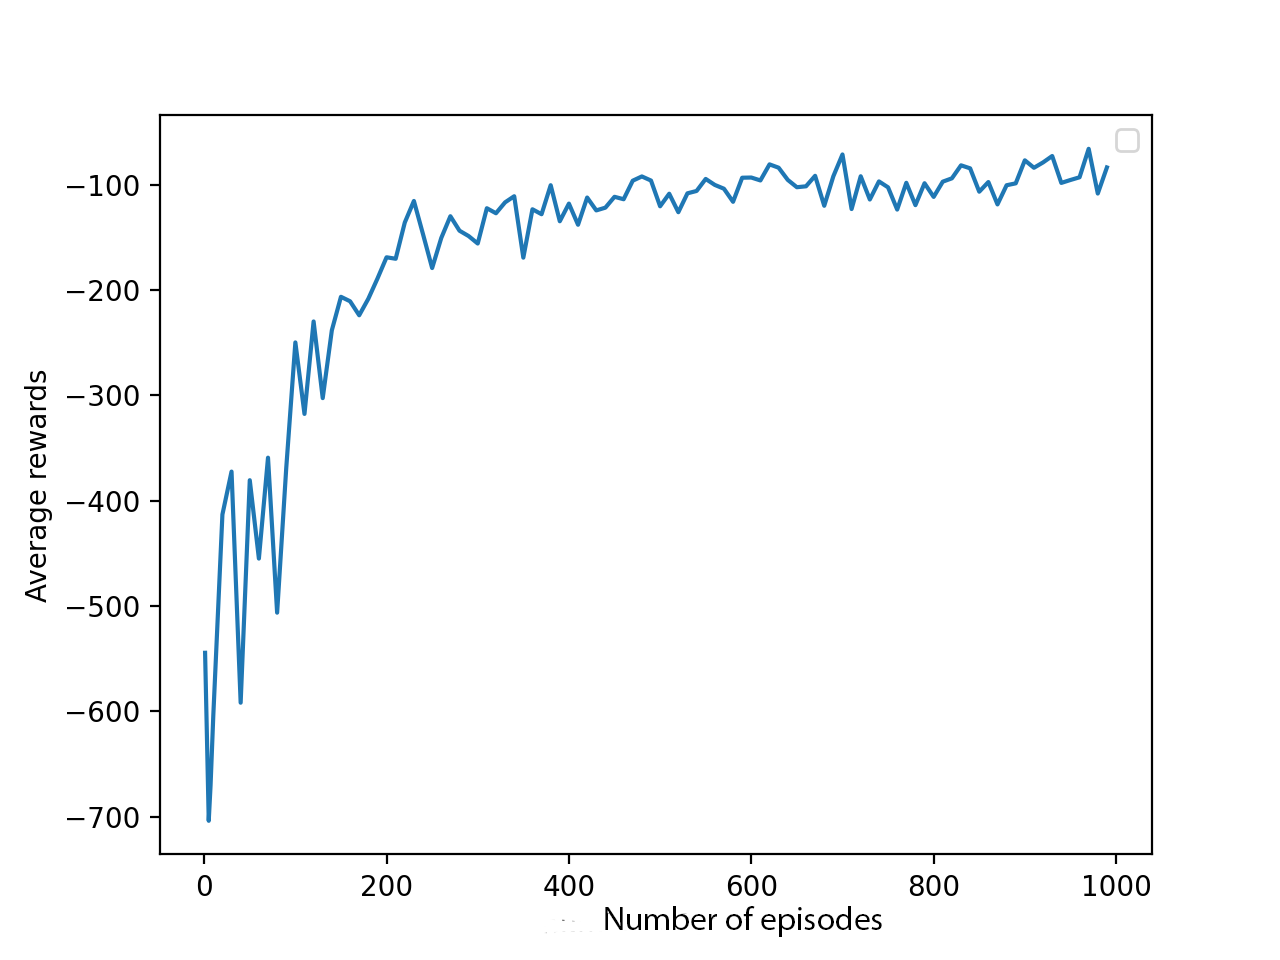
\includegraphics[scale = 0.5]{2.png}
  \caption{Average rewards of 50 simulations in first 1000 episodes}
\end{figure}

Figure 3 below shows the optimal path starting from [10,0], [14,0] and [19,0] until they runs out of the map. It is interesting that the car will reach finishing line starting form [10,0] and  [14,0], but runs out of the track directly starting from [19,0]. There are two possible explanation of this 1) This is indeed the optimal policy, the car will get to finishing line faster starting from other points 2) We haven't repeat the simulation for enough episodes, so the action is not actually not optimal.†

\begin{figure}
  \centering
     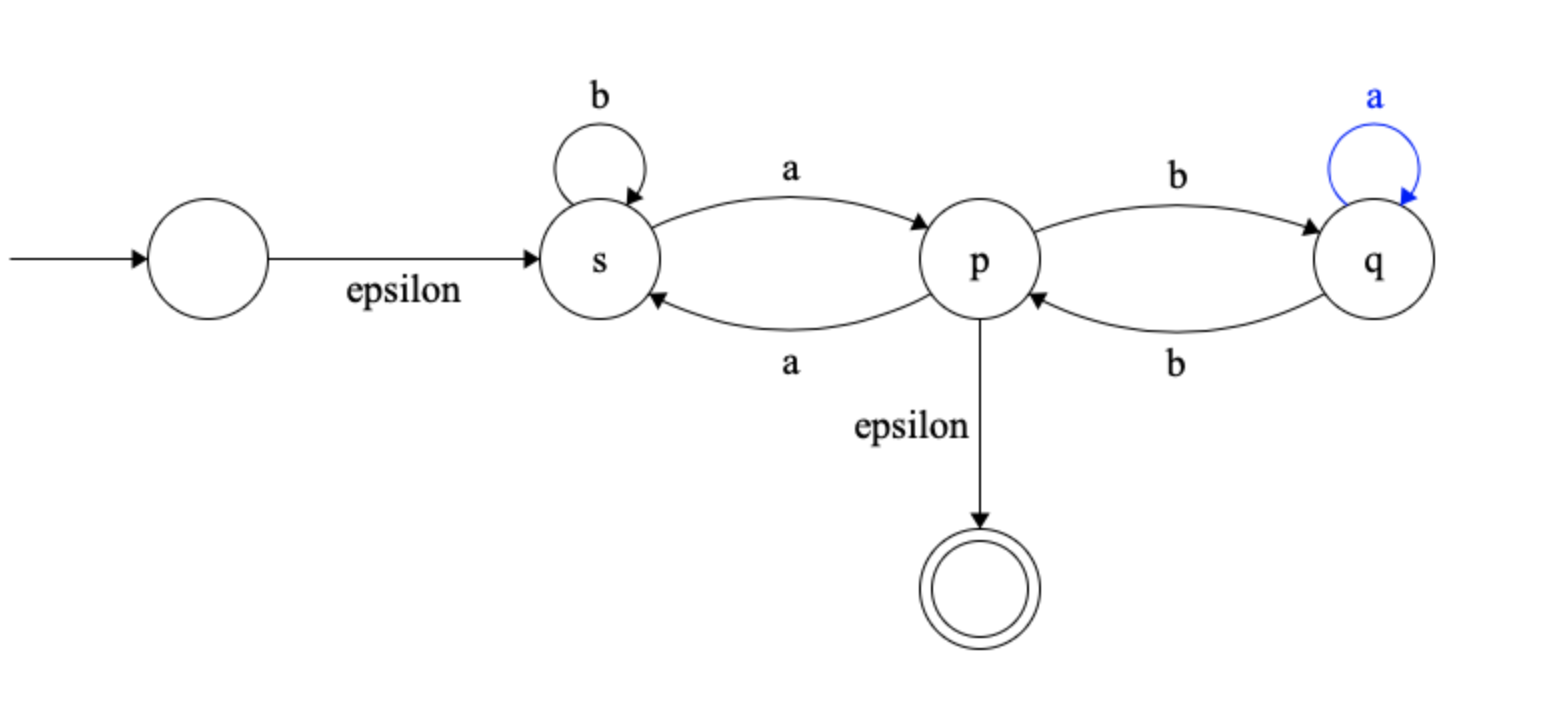
\includegraphics[scale = 0.24]{3.png}
  \caption{optimal path starting from [10,0], [14,0] and [19,0] until they runs out of the map}
\end{figure}

\pagebreak

\section{Further Experiment}
Here, we try to expand the track (see figure 4) and try to transfer the data we got from original problem to this problem.\\
We can see from Figure 5 that original data indeed helps in finding optimal path in the new track.


\begin{figure}
  \centering
     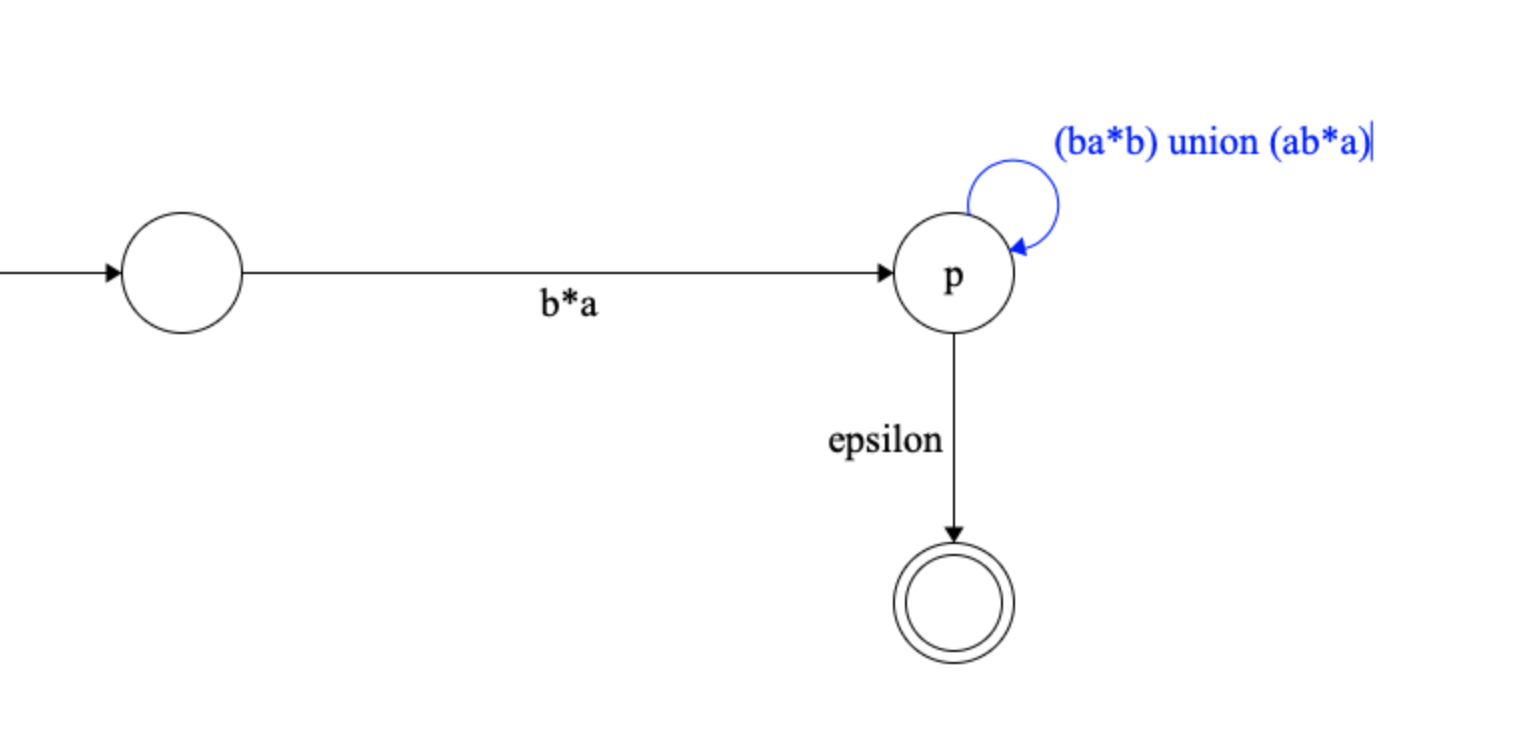
\includegraphics[scale = 0.16]{5.png}
  \caption{Race Track drawn in grid, yellow areas are starting line and finish line, this can be viewed as an expansion of the original track}
\end{figure}

\begin{figure}
  \centering
     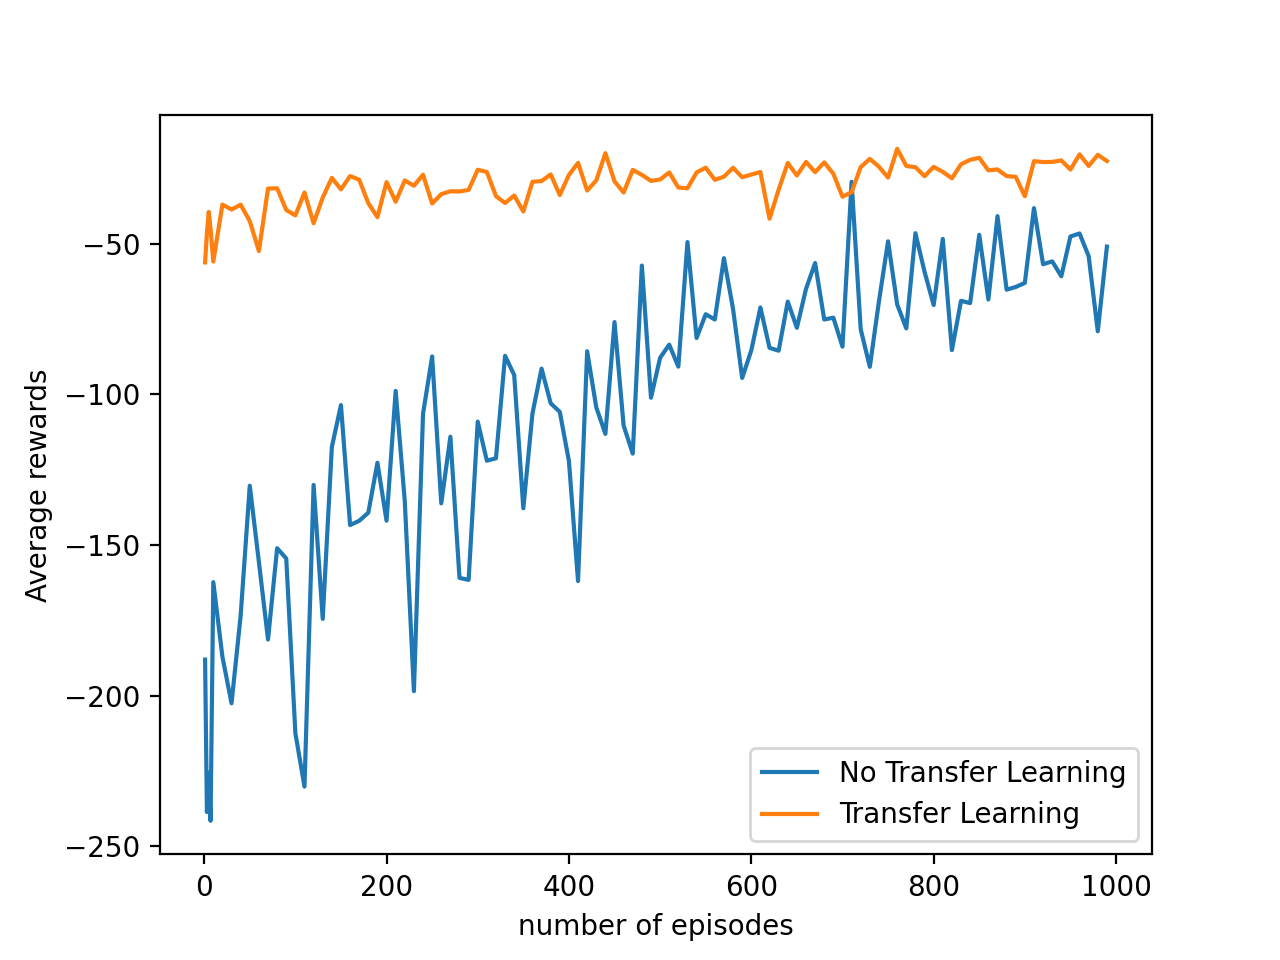
\includegraphics[scale = 1.0]{10.png}
  \caption{Average rewards of 20 simulations in first 1000 episodes for Monte-Carlo with knowledge transferred(orange) and Monte-Carlo without knowledge transferred(blue)}
\end{figure}

\pagebreak

\section{Extra Credit Work}
\subsection{Exercise 4.4}
We want to modify the policy so its termination is guaranteed since the policy  may never terminate if the policy continually switches between two or more policies that are equally good.  We could add a comparison on the expected value of two policies. and only change policy if new policy is strictly better than original policy.\\
So we only need to change the policy improvement part of the algorithm:\\

(1)$policy$-$stable \leftarrow true$\\
(2)For each $s \in S$:\\
(3)\qquad$old$-$action\leftarrow\pi(s)$\\
(4)\qquad$\pi'(s) \leftarrow \Sigma_{s',r} p(s',r|s,a)[r + \gamma V(s')]$\\
(5)\qquad If $\Sigma_{s',r} p(s',r|s,\pi'(s))[r + \gamma V(s')] > \Sigma_{s',r} p(s',r|s,\pi(s))[r + \gamma V(s')]$:\\
(6)\qquad\qquad $\pi(s) \leftarrow \pi'(s)$ \\
(7)\qquad If old-action $\ne \pi(s)$, then $policy$-$stable\leftarrow false$  \\
(8)If $policy$-$stable$, then stop and return $V\approx v_* and \pi \approx \pi_*,$else go to (2)\\


\subsection{Exercise 5.1}
The estimated value function jump up for the last 2 rows in the rear because the player has 20 or 21 and he stop taking cars and has a high chance of winning\\

The diagram drop off for the whole last row on the left is because the dealer shows an ace so the player is less likely to win.\\

The frontmost values are higher in the upper diagrams than in the lower because the player has a usable ace, which makes him more likelyto win.

\pagebreak


\end{document}

